\documentclass[conference]{IEEEtran}
%\documentclass{article}
\usepackage{setspace}
\spacing{0.94}
\usepackage[cmex10]{amsmath}
\usepackage{algorithm}
\usepackage{algpseudocode}
\usepackage{array}
\usepackage{url}
\usepackage{graphicx}
\usepackage{pbox}
\usepackage{hyperref}


\usepackage{amsfonts}
\usepackage{varwidth}
\algnewcommand\algorithmicforeach{\textbf{for each}}
\algdef{S}[FOR]{ForEach}[1]{\algorithmicforeach\ #1\ \algorithmicdo}

%\usepackage{romannum}
\makeatletter
\newcommand{\rmnum}[1]{\romannumeral #1}
\newcommand{\Rmnum}[1]{\expandafter\@slowromancap\romannumeral #1@}
\makeatother

\usepackage{setspace}
%\singlespacing
%\onehalfspacing
%\doublespacing
\hyphenation{op-tical net-works semi-conduc-tor}

\begin{document}

\title{Secure Sharing of Private Locations through Homomorphic Bloom Filters}



% make the title area
\maketitle

% As a general rule, do not put math, special symbols or citations
% in the abstract
\begin{abstract}
Location information is becoming increasingly popular in online social networks, vehicle networks, and online games. In this paper, we develop a distributed protocol that allows one party to determine, in a private and secure manner, whether or not the trajectory of a second party has an intersection with the first party. Our design is fully flexible, meaning that each user is able to specify what kind of datasets they would like to make visible, and be queried by other users. The methodology is based on developing a generalized set membership check approach, where our design is based on an advanced data structure called the bloom filter. Our work, to our knowledge, is the first to propose a homomorphic version of this data structure.  To demonstrate its feasibility, we offer a working prototype, which is implemented on the open-source homomorphic libraries. Our preliminary results demonstrate the performance and overhead of the proposed approach as well as the security of the protocol designs.
\end{abstract}

% no keywords

% For peer review papers, you can put extra information on the cover
% page as needed:
% \ifCLASSOPTIONpeerreview
% \begin{center} \bfseries EDICS Category: 3-BBND \end{center}
%
% For peerreview papers, this IEEEtran command inserts a page break and
% creates the second title. It will be ignored for other modes.
%\IEEEpeerreviewmaketitle



\section{Introduction}
\label{sec:introduction}

Location information is becoming increasingly popular in online social networks, vehicle networks, and online games. Companies like Google and Uber have heavily invested in autonomous vehicles that make driving decisions based on real-time highly accurate location coordinates~\cite{markoff2010google}. On smartphones, more users are sharing location data through multiple types of apps, ranging from navigation maps to geographically enhanced games, such as the hugely popular game Pokemon Go~\cite{pokeman}. In these scenarios, one big concern has been the privacy of users, as unexpected leaks of users' location trajectories will allow potentially malicious attacks to gain advantages in the real-world~\cite{locationprivacy}. For example, by knowing when a user leaves and returns home each day, a potential third-party attacker could identify the time periods during which the user’s home is not occupied.  The attacks range from mild inconveniences such as privacy leaks to much more serious attacks such as break-ins, among other types of attacks.

One significant challenge on keeping location data secure is that we should not trust servers as safe against attacks~\cite{krutz2010cloud}. Indeed, the significant increase on hacking activities against servers in recent years~\cite{liao2013intrusion,grispos2013calm} means that if we store non-encrypted data on servers, we will face the risks that such data may be leaked when the severs themselves compromised. Perhaps paradoxically, when building apps that involve location data, servers typically perform extensive computation on the location traces, making it necessary for the servers to be able to decrypt data as needed. For example, Google Maps needs to obtain the starting and ending locations to calculate the trajectories for navigation purposes, and Facebook servers need users' geographic regions to accurately deliver targeted advertisements. So the challenge is, is it still possible for us to maintain security of location traces while \emph{allowing} servers to perform app-specific computations?

Given the demands from users to keep their location data secure, as well as the need for the servers to perform basic operations on the trajectory data, in this paper, we investigate methods such that we can achieve both goals simultaneously. Specifically, we develop secure computation primitives on location data where the servers should have no knowledge on the plaintext, i.e., the servers should not even keep the private keys to decrypt data. In this way, compromised servers will not cause leaked user data. Our work is motivated and enabled by the recently developed homomorphic computing principles: recent advances in this area has demonstrated it is feasible to perform meaningful and predictable computations on encrypted data without decrypting them first~\cite{Gentry:2009:FHE:1536414.1536440,ahn2015computing}. In our work, we build on these homomorphic principles, and focus on one commonly used primitive in location data processing: computing the intersections between location datasets. Such a primitive can be used for many apps, ranging from deciding if users' trajectories match query requirements for targeted advertisement deliveries, to suggesting the most appropriate users for ride-sharing purposes.

Specifically, our computational primitive works as follows: we consider two users, Alice and Bob, to find out if their location datasets (e.g., such sets could be collections of singleton locations, or continuous trajectories, or areas within specified boundaries) have intersections. The application model is as follows: Alice can publish her location dataset after encrypting them first, via an aggregation server (e.g., her Facebook page), meaning that Bob does not get access to the data directly. Instead, Bob can send a query to the aggregation server by using his location sets as the query key. Note that as Bob also cares about his privacy, Alice should not see the plaintext of Bob’s location set neither. Hence, Bob should avoid sending plaintext in the query. Next, the aggregation server performs the \emph{matching} step, where Alice's secured datasets are matched against Bob's query, and a (still encrypted) computational result is returned to Alice. Alice can decide whether there is an intersection between the incoming query and her datasets by decrypting the result using her own private key. If there is an intersection, Alice is able to send additional information to Bob, possibly through the help of the aggregation server since it knows Bob's identity (e.g., social media accounts or emails).

We now make a few remarks on this computational model. First, by design, this model ensures that the location datasets are fully secure, as Alice will only publish the datasets that are encrypted using her public key. On the side of Bob, as we will explain later, the plain text is also processed using hash functions. By choosing sufficiently strong cryptographic hashing functions, we can also ensure that the plain text of Bob is well protected. Hence, Alice and Bob do not directly share the plaintext of their location histories. Second, this computational model is sufficiently secure against compromised servers, as the aggregation server does not keep any plaintext of location trajectories. Finally, only queries that return positive results (i.e., there are intersections) will lead to further interactions between Alice and Bob.

The central methodology in our implementation is based on an advanced data structure called the bloom filter, which has been widely adopted in the networking literature~\cite{broder2004network}. Our work, to our knowledge, is the first to propose a homomorphic version of this data structure. In our design, we offer both a standard form design as well as two optimized designs, and compare their performance. Figure~\ref{fig:architecture} shows an overview of the proposed framework, where the actions taken by Alice, Bob, and the aggregation server are illustrated. 

\begin{figure}[t]
	\centering
	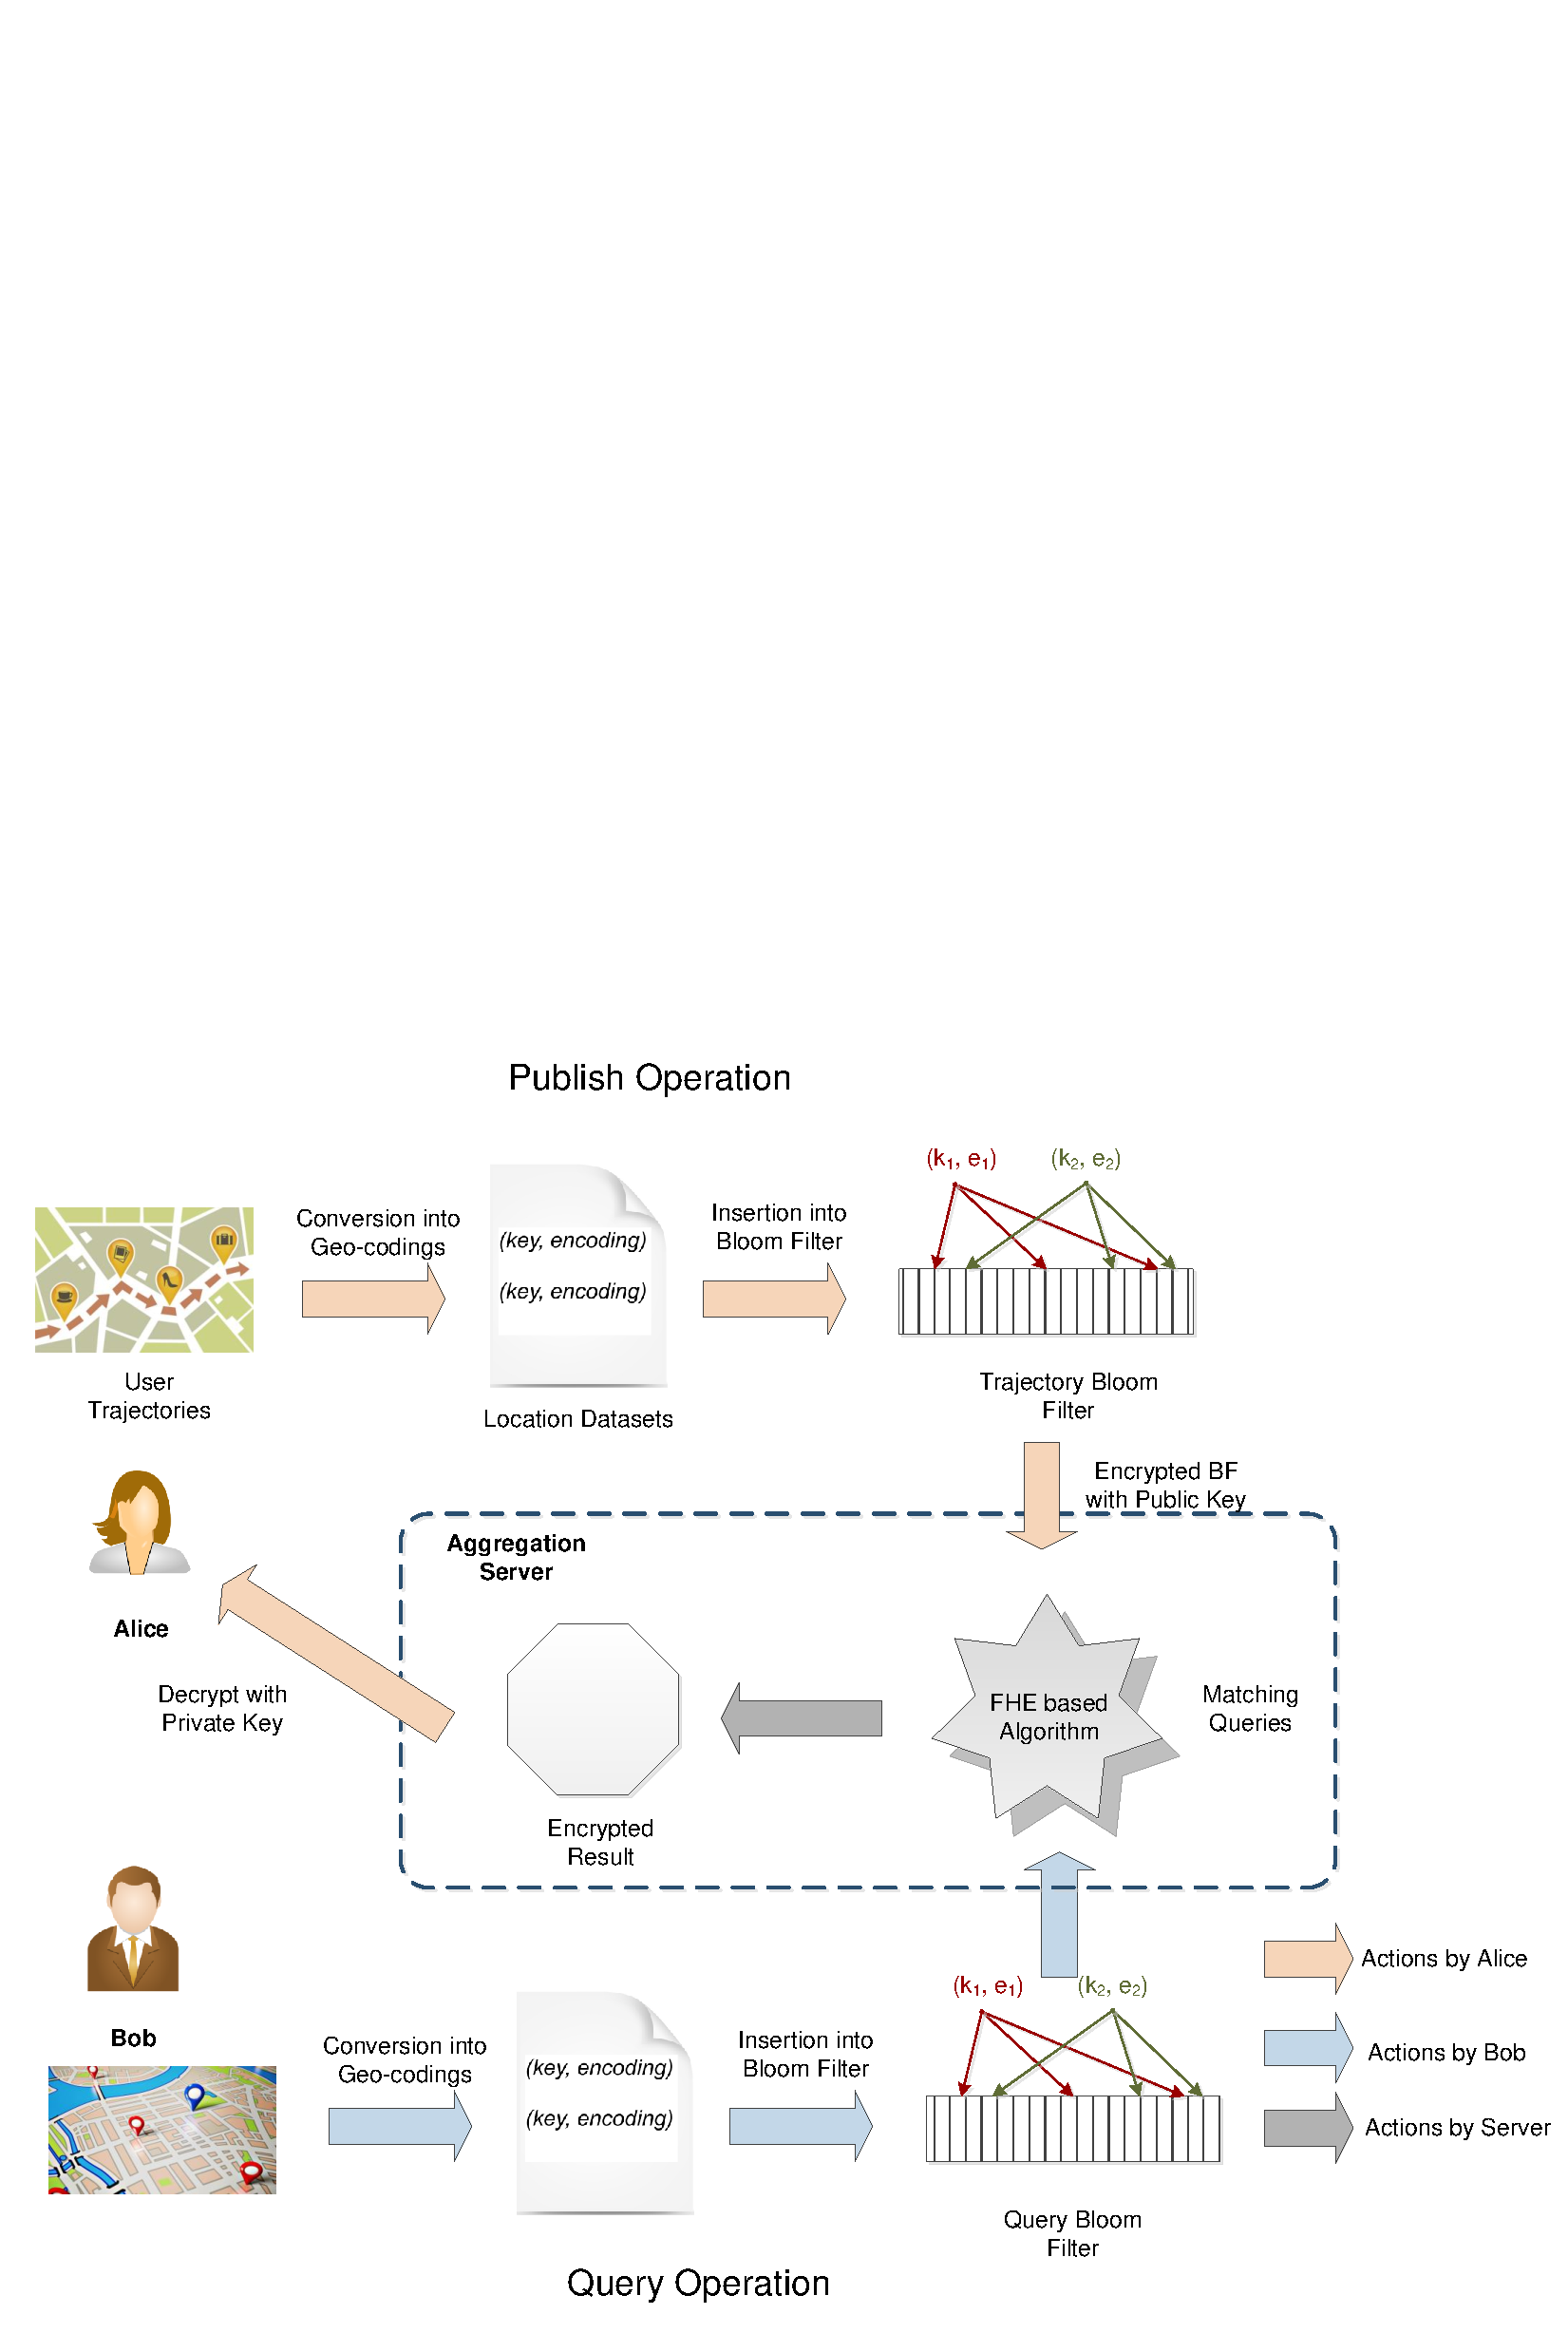
\includegraphics[width=0.8\linewidth]{figures/architecture.pdf}
	%\vspace{-0.1in}
	\caption{Computational model architecture}
	\label{fig:architecture}
	\vspace{-0.1in}
\end{figure}


Another major contribution of this paper is that we develop a distributed protocol that allows one party to determine, in a private and secure manner, whether or not a second party's trajectory has an intersection with the first party. Our design is fully flexible, meaning that each user is able to specify what kind of datasets they would like to make visible, and be queried by other users. The location datasets can include trajectories, areas, and isolated points. For areas, we also present a geohash based optimization that allows areas to be represented in a compact and flexible manner. 

The third contribution this paper is that we offer a working prototype, which is implemented on the open-source homomorphic libraries. Our preliminary results demonstrate the feasibility of the proposed approach as well as the security of the protocol designs. We also evaluate the performance of our implementation with a real-world dataset that is collected in a city area on users' smartphones to demonstrate the effectiveness of large-scale location queries.

The remaining of this paper is organized as follows. In Section 2, we describe the related work to our paper. In Section 3, we describe the problem formulation and the protocol design. In Section 4, we describe the prototype design and implementation details. In Section 5, we describe the analysis of security. In Section 6, we describe the evaluation results. In Section 7, we describe the conclusions.

\section{Related Work}
\label{sec:related}

The security of location data has been closely investigated in the previous literature~\cite{fawaz2014location,gibler2012androidleaks}, as such data can be used to identify a wide range of activities and valuable information of the carrier for tracking purposes~\cite{farrahi2010probabilistic}. For example, previous research has demonstrated that it is possible to reconstruct transportation modes of users through their location data alone~\cite{bierlaire2013probabilistic}. Meanwhile, recent rises on attacks on servers and information leaks indicate that we could not trust the service providers for keeping vital data secure~\cite{vasek2016hacking}. Therefore, we should find ways to store and process location data in a secure and trustworthy manner.

Previous work on keeping location secure has investigated multiple directions. The first direction, which is called k-anonymous obfuscation~\cite{casino2015k,phan2015kur}, tries to hide the true locations of users by obfuscating them to the granularity of larger cells. Such methods, although protecting privacy, make it harder to develop applications that require the precise locations of users. Another method is through statistical methods~\cite{seidl2015spatial}, which add random noise to the samples of individual users, but keep the global statistical parameters to be more or less reliable. Again, such methods are only suitable for large-scale statistical needs but are not useful where one user's data needs to be exploited for application needs, e.g., ride sharing, targeted promotions, and navigations. 

There has also been work to study the private equality test~\cite{kotzanikolaou2016lightweight, patsakis2015private}, where two parties A and B wants to conclude whether they have the same number privately. The private location equality test can be easily reduced to this problem. The private location equality test, however, does not support comparing with multiple locations, hence can be considered as a very special case of the problem we are studying. 

In order to achieve location security and privacy,  we must perform encryption and decryption methods on the location data, so that users can be secure when servers may be compromised. We adopt well known public-key based encryption methods in our work. Based on the encrypted data, we apply the ideas from the recently proposed homomorphic encryption, which aims to perform complex processing on the encrypted data, yet still yielding results that, once decrypted, are meaningful and correct results on the user side. The ideas of homomorphic computing have been proposed in the literature for several decades, but only in the past several years practical methods have been developed to prove the feasibility of these goals~\cite{Gentry:2009:FHE:1536414.1536440, van2010fully, brakerski2011fully, brakerski2014efficient, brakerski2012leveled, fan2012somewhat, lopez2012fly, brakerski2012fully, bos2013improved, gentry2013homomorphic, brakerski2014lattice}. We therefore build our protocol on top of representative homomorphic computing libraries,  but we note that future developments of better paradigms will lead to lower computing cost and overhead, as well as better security in our system. More specifically, recently there have been two types of homomorphic encryption methods proposed, including the fully homomorphic encryption methods (FHE)~\cite{Gentry:2009:FHE:1536414.1536440, van2010fully, brakerski2011fully} and the somewhat encryption methods~\cite{brakerski2014efficient, brakerski2012leveled, fan2012somewhat, lopez2012fly, brakerski2012fully, bos2013improved, gentry2013homomorphic, brakerski2014lattice}.  While the FHE methods provide support for arbitrary number of operations, the second type only supports a  limited types of operations. Our used libraries fall under the second category, as the FHE methods are still under research due to their excessive demands on computational costs. 

\section{Design}
\label{sec:design}

In this section, we describe the assumptions, design, and optimization of the protocol.

\subsection{Assumptions}

Our system design consists of three parties: Alice, Bob, and the aggregation server. In a typical application scenario, Alice may selectively publish her location datasets after encrypting them with her public key. Later, another user Bob queries on the location trajectories of Alice. The aggregation server is responsible to perform computation tasks on the encrypted data, and sends the (still encrypted) results to Alice. Alice is able to decide whether the query has intersection with the published data. If the query returns false, Alice is not able to learn about Bob’s location either.

We next describe what we mean by location datasets. Specifically, each user is able to represent their locations with GPS coordinates using tuples (latitude, longitude). One user may either specify a trajectory through consecutive tuples, or an area with tuple boundaries (e.g., a polygon or a circle). The goal of the aggregation server is that it is able to broadcast the encrypted location sets. To achieve this, each user also maintains a pair of public and private keys. Every bit of data, when sent to the server, will be encrypted using the public key to ensure security.

On the user side, we assume that Alice and Bob are usually not malicious. They will follow the protocol correctly but once the protocol has ended they can perform any computation they want on the information (encrypted or otherwise). If Alice finds out that there is an intersection with the trajectory of the query, the further interactions between Alice and Bob are out of scope of this protocol.


\subsection{Background}

We first describe the background of our work as follows.

\textbf{Homomorphic Cryptography:} Homomorphic encryption takes a foundational role in our system. Briefly, in fully homomorphic encryption~\cite{fan2012somewhat} and~\cite{van2010fully}, the following equations hold true:
\vspace{-0.1in}
\begin{equation}
m_1 + m_2 = D(E(m_1) + E(m_2))
\end{equation}
\begin{equation}
m_1 * m_2 = D(E(m_1) * E(m_2))
\end{equation}

In these equations, $E()$ stands for the encryption, $D()$ stands for the decryption. Computation can be done with encrypted values that translates to operations in the plain text domain. This allows parties to perform blind computation on encrypted values. In our design, we mostly rely on the addition operation rather than the multiplication operation due to the efficiency concerns.

\textbf{Bloom Filter:} We use standard notations on bloom filters to represent their operations, as follows:

\begin{itemize}
\item $m$: the total number of bits in the bloom filter;
\item $k$: the number of hash functions;
\item $n$: the number of elements inserted in the bloom filter;
\item $p$: false positive probability of the bloom filter;
\item $t$: the number of bits set to one.
\end{itemize}

The probability of false positives $p$ given a parameter set is:
\vspace{-0.1in}
\begin{equation}
p = (1-e^{\frac{-kn}{m}})^k
\label{equ:p}
\end{equation}

For a given $m$ and $n$, the value of $k$ that minimizes the false positive is:
\vspace{-0.1in}
\begin{equation}
k = \frac{m}{n}\ln2
\label{equ:k}
\end{equation}

For a given $n$ and the desired false positive $p$, the required number of bits $m$ is:
\vspace{-0.1in}
\begin{equation}
m = - \frac{n\ln p}{{(\ln2)}^2}
\label{equ:m}
\end{equation}


%For a given $m$, $k$ and $t$, the estimated elements in bloom filter is:

%\begin{equation}
%n* = - \frac{m\ln [1 - \frac{t}{m}]}{k}
%\label{equ:n}
%\end{equation}

We use these results later for performance analysis of our protocol.

\subsection{Main Protocol Idea with FHE}

The main idea for the protocol works as follows. The user Alice first inserts all locations as inputs to a configured bloom filter $BF$, by hashing locations to $k$ positions, and flipping corresponding bits. After all locations are inserted, suppose that this filter has $m$ bits, and $t$ bits have been set as $1$s, whose locations are specified as $b_1$,$b_2$,..., $b_t$. Our next goal is to encrypt the bloom filter $BF$ properly. Specifically, we observe that its set bits can be represented as a polynomial as:

\begin{equation}
\vspace{-0.1in}
f(x) = \prod_{i=1}^{t} (x-b_i)
\end{equation}

Alice then sends the encrypted polynomial $f(x)$ either in the product form or in the extended form to the aggregation server. Alice also sends the details on the $k$ hash functions, as well as the configuration parameters for the bloom filter. This is necessary as such information will later used by Bob for encryption needs as well. Even though A sends the hash functions, as the $f(x)$ is encrypted with the public key, the aggregation server has no way to learn which bits have been set as $1$ in the bloom filter.

The aggregation server next waits for the query from Bob. However, Bob does not send the query, i.e., locations, in plain text either. Instead, Bob will first obtain the $k$ hash functions from the server, and hash the query locations into $k$ bits as $p_1$, $p_2$, $\cdots$, $p_k$. Bob would like to test if all these bits have been set as $1$ in the encrypted bloom filter sent by Alice. To do this, Bob sends the $k$ positions to the server, which then can calculate for each location, whether the polynomial has a corresponding bit set as $1$. To do this, we can test each of the $k$ positions individually, by evaluating of $f(x)$ in the encrypted form as $E(f(p_i))$. We know that, based on the nature of this encryption method, the following equation also holds true:

\begin{equation}
\vspace{-0.1in}
D(E(f(p_i))) = f(p_i)
\end{equation}

Furthermore, if $p_i$ has been flipped to $1$ by Alice earlier, this evaluation result must be $0$ based on the product nature of the polynomial. Therefore, if we construct another polynomial as $\sum_{i=1}^{k}(E(f(p_i)^2)$ (we use square is to prevent the evaluation may sometimes lead to negative numbers), we have:

\begin{equation}
\vspace{-0.1in}
H(p) = D[\sum_{i=1}^{k}(E(f(p_i))^2] = \sum_{i=1}^{k}(f(p_i)^2)
\end{equation}

Observe that in this equation, only when all $k$ bit locations have been flipped to $1$, the result $H(p)$ will be $0$. If $H(p)$ is not $0$, then it means that the query is not in the bloom filter. We note that the multiplication steps for computing $H(p)$ is $t$ (based on the factorized form of $f(x))$, the total time of multiplication involved is $O(k*t)$. A large $t$, like 200, makes such a multiplication impractical for two reasons: first, the fast growth of ``inherent noise'' in ciphertexts of FHE schemes makes them likely to be corrupted very quickly, which limits the computation capacity greatly; second, the fast increased size of ciphertexts worsens the computation overhead. Some techniques, such as relinearization~\cite{brakerski2012leveled} and approximate eigenvector method~\cite{gentry2013homomorphic}, have been proposed to balance the multiplication computation capacity and computation overhead, but they still do not work efficiently on a huge multiplication depth in real applications. So, we design the following alternative protocols containing limited or no multiplication operations. We call these protocols \emph{practical} for this reason.




\subsection{Practical Protocol 1: An Improved Implementation of the Homomorphic Bloom Filter}
\label{subsec:basic_implementation}

We now describe the first working implementation using fewer additions and multiplications compared to the primitive idea above. Its pseudocode is shown in Algorithm \ref{alg1}. Alice first inserts her locations into a bloom filter $BF$ using $k$ hash functions, where $t$ bits have been set as $1$, and the corresponding positions are specified as $b_1, b_2, \dots, b_t$. Then Alice uses her public key $PK$ to encrypt each negated $b_i$ as the encrypted $E(-b_i)$, which are then submitted to the aggregation server. After launching a query, Bob first asks the public key $PK$ and the same $k$ hash functions from Alice. Then Bob hashes his query location into k bits as $p_1, p_2, \dots, p_k$, which are then encrypted as $E(p_1), E(p_2), \dots, E(p_k)$ by $PK$ and submitted to the same aggregation server. Once receiving the encrypted query from Bob, the server starts the evaluation based on $E(b)$ and $E(p)$. Specifically, for each $E(p_j)$, the server performs $E(p_j) + E(-b_i)$, where $i = 1, 2, \dots, t$, and gets $t$ encrypted results which are then decrypted as $D(E(p_j) + E(-b_i))$ respectively by Alice using her secret key $SK$. Notice that in this design, the information of Bob might still be leaked to Alice no matter whether they have trajectory intersections or not, because Alice can obtain the value of $p_j$ by:
\begin{equation}
p_j =\frac{\sum_{i = 1}^{t}[D(E(p_j) + E(-b_i)) + b_i]}{t}
\end{equation}

To address this problem, we introduce the randomness during the evaluation by multiplying $E(p_j) + E(-b_i)$ by a random positive integer $z$. Thus, if $D(E(p_j) + E(-b_i))$ equals 0, $D((E(p_j) + E(-b_i))*z)$ still equals 0, while other values vary dramatically. Once one of the $t$ encrypted results of $p_j$ equals 0, it means the position of $p_j$ in $BF$ is set as 1. If all positions of $p_j$ for $j$ from $1$ to $k$ in $BF$ is set as 1, we can conclude Bob has an interaction with Alice with a certain confidence level which are determined by $BF$'s rate of false positives (we analyze the impact of this false positive rate later). Otherwise, Bob has no intersection with Alice at the query location $100\%$.


\begin{algorithm}\small
\caption{A Basic Implementation of the Homomorphic Bloom Filter}
\label{alg1}
\begin{algorithmic}[1]

\Statex Alice: Bloom Filter Encryption
\State $b \gets BF.get\_ones\_positions()$
\For{$i = 1 \to t$}
    \State $E(-b_i) \gets$ encrypt $-b_i$ using $PK$
\EndFor
\State send $E(-b)$ to the aggregation server

\item[]

\Statex Bob: Query Encryption
\State $p \gets$ hashed value of his location
\For{$j = 1 \to k$}
    \State $E(p_j) \gets$ encrypt $p_j$ using $PK$
\EndFor
\State send $E(p)$ to the aggregation server

\item[]

\Statex Sever: Evaluation
\For{$j = 1 \to k$}
    \For{$i = 1 \to t$}
        \State $cipher\_result_{ij} \gets (E(p_j) + E(-b_i))*z$
    \EndFor
\EndFor
\State send $cipher\_result$ to Alice

\item[]

\Statex Alice: Result Decryption
\For{$j = 1 \to k$}
    \State $flag \gets FALSE$
    \For{$i = 1 \to t$}
        \State $plain\_result_{ij} \gets$ decrypt $cipher\_result_{ij}$ using $SK$
        \If {$plain\_result_{ij} = 0$}
            \State $flag \gets TRUE$
            \State \textbf{break}
        \EndIf
    \EndFor
    \If {$flag = FALSE$}
        \State \textbf{return} no intersection
    \EndIf
\EndFor
\State \textbf{return} intersection exists

\end{algorithmic}
\end{algorithm}



\subsection{Practical Protocol 2: A Lightweight Evaluating Implementation of the Homomorphic Bloom Filter}
The previous protocol requires $k*t$ additions and one-depth multiplications respectively for evaluation and $k*t$ times of decryptions in the worst case, which may pose a burden on the speed of query. In this section, we propose an improvement that requires $k$ additions, no multiplication and one decryption to speedup the query. The pseudocode is shown in Algorithm \ref{alg2}. Like protocol 1, Bob queries Alice's locations. After inserting her locations into the bloom filter $BF$, Alice encrypts every bit, $b_1, b_2, \dots, b_m$, in $BF$ and submits $E(b)$ to the aggregation server. Then Bob uses the same $k$ hash functions Alice uses to hash his query location into $p_1, p_2, \dots, p_k$ which actually are the corresponding bit positions in $BF$. These hashed values $p$ are submitted to the server in plaintext, which we think is still safe because the chosen $k$ cryptohash functions ensure that the server cannot reversely compute the plain text from hashed values. The server then sums all elements in $E(b)$ whose index is in $p$. Then the server subtracts $k$, i.e., the length of $p$, from the sum and returns the cyphertext result to Alice for decryption. The whole evaluation and decryption can be expressed as follows:

\begin{equation}
plain\_result = D(\sum_{j = 1}^{k}E(b_{p_j}) - E(k))
\end{equation}

If $plain\_result$ equals 0, it implies that all values of $b_{p_j}$ are same and equal 1. In other words, all positions of $p_j$ in $BF$ are flipped as 1. So, we can say Bob interacts Alice with a certain probability of false positive expressed by Equation \ref{equ:p}. Otherwise, they do not intersect at the query location 100\%.

\begin{algorithm}\small
\caption{A Lightweight Evaluating Implementation of the Homomorphic Bloom Filter}
\label{alg2}
\begin{algorithmic}[1]


\Statex Alice: Bloom Filter Encryption
\State $b \gets BF.get\_all\_elements()$
\For{$i = 1 \to m$} \Comment{$m$ is the size of $BF$}
    \State $E(b_i) \gets$ encrypt $b_i$ using $PK$
\EndFor
\State send $E(b)$ to the aggregation server

\item[]

\Statex Bob: Query Encryption
\State $p \gets$ hashed value of his location
\State $E(k) \gets$ encrypt $k$ using $PK$
\State send $E(k)$ and $p$ to the aggregation server

\item[]

\Statex Sever: Evaluation
\State $sum \gets 0$
\For{$j = 1 \to k$}
    \State $sum \gets sum + E(b_{p_j})$
\EndFor
\State $cipher\_result \gets sum - E(k)$
\State send $cipher\_result$ to Alice

\item[]

\Statex Alice: Result Decryption
\State $plain\_result \gets$ decrypt $cipher\_result$ using $SK$

\end{algorithmic}
\end{algorithm}


\subsection{Practical Protocol 3: A Bit-wise Implementation of the Homomorphic Bloom Filter}

\begin{figure}[t]
    \centering
    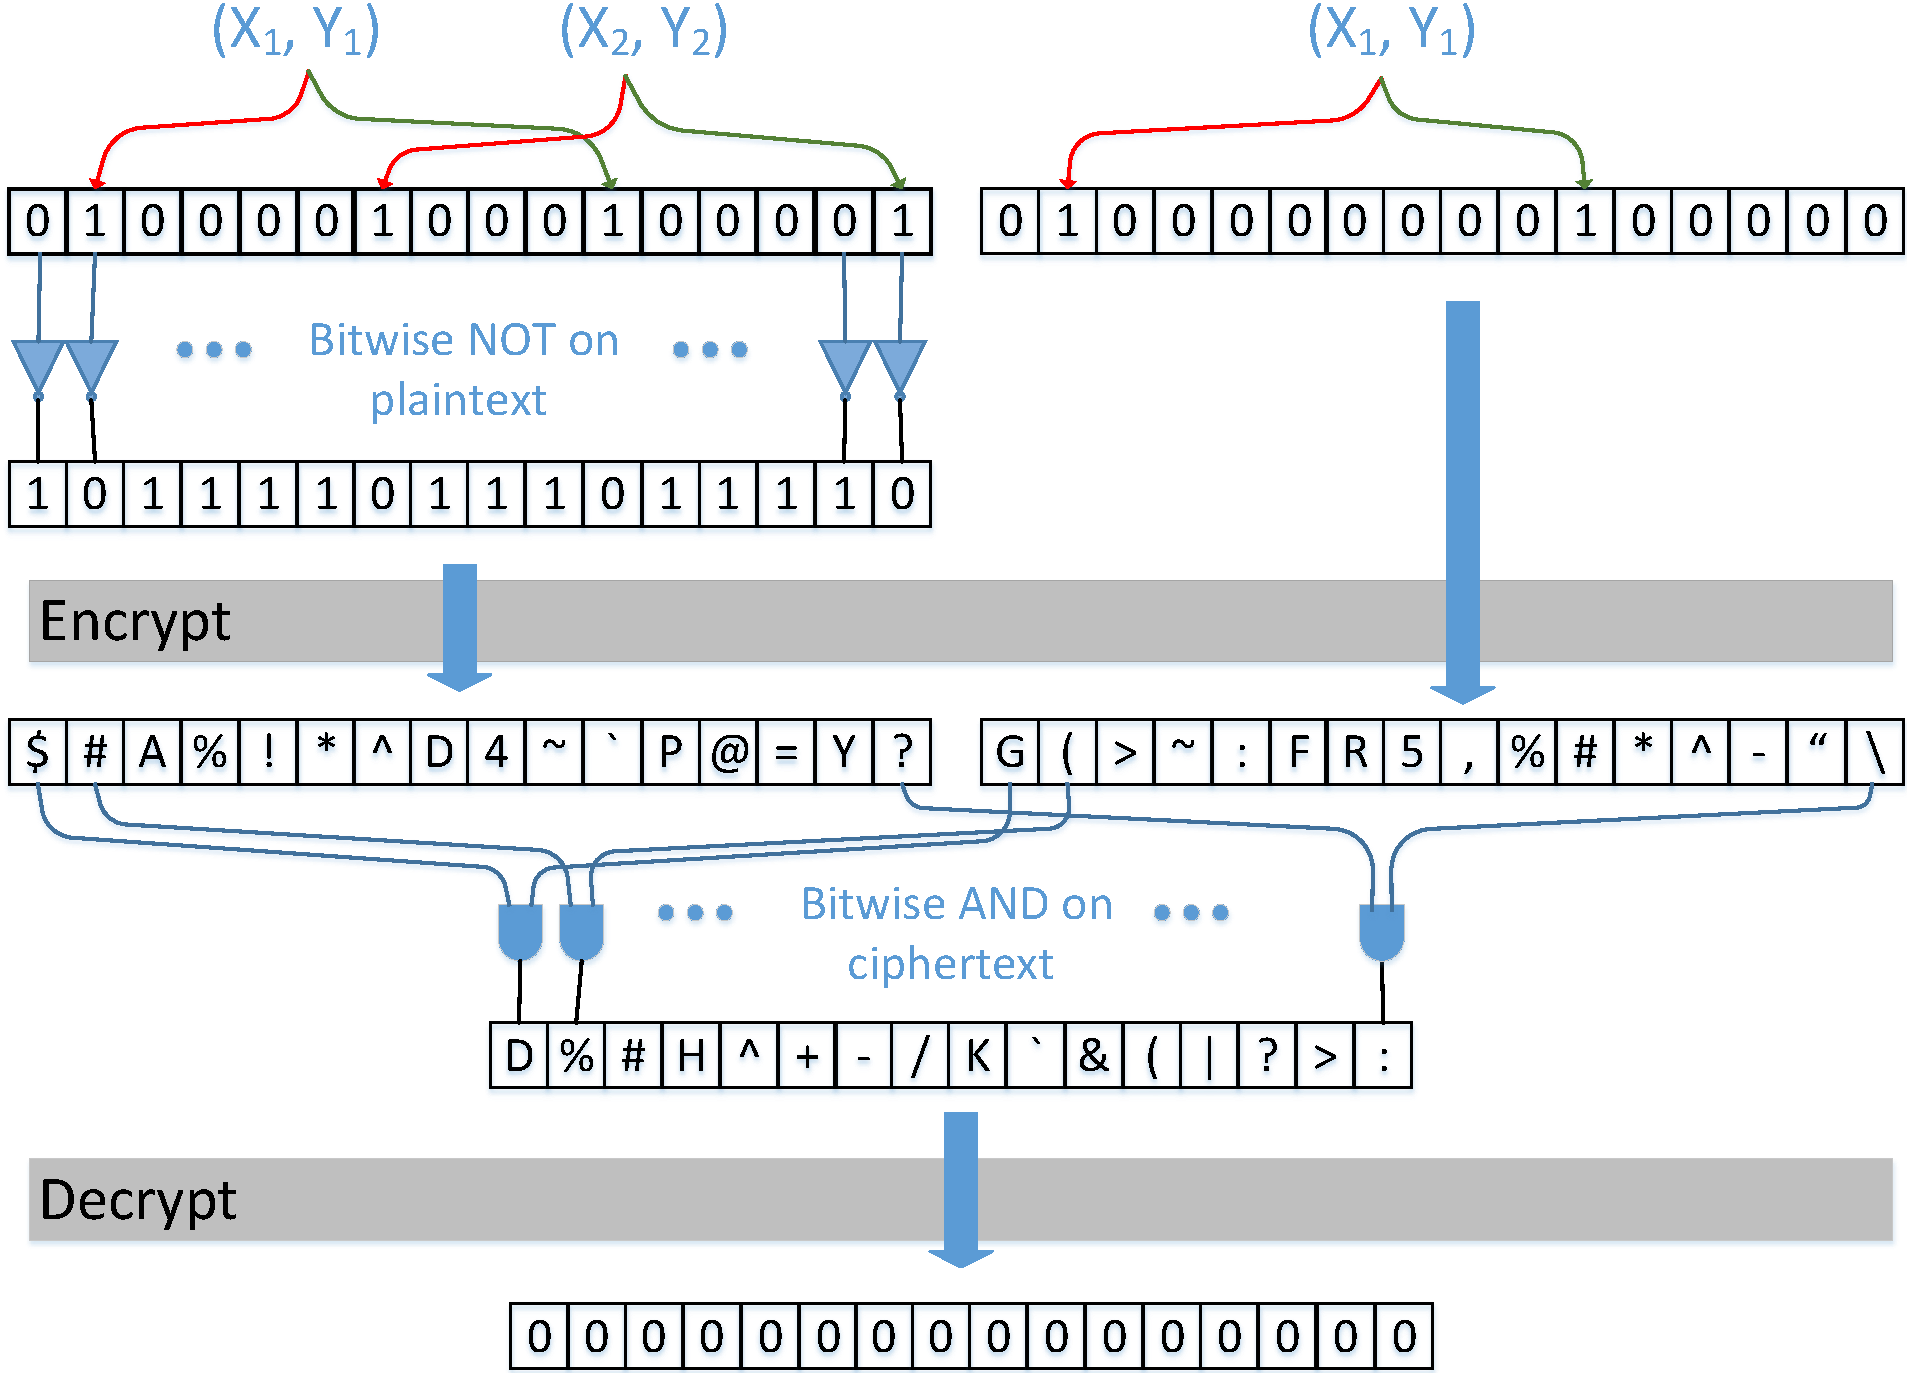
\includegraphics[width=0.8\linewidth]{figures/bitwise_bloomfilter.pdf}
    %\vspace{-0.1in}
    \caption{Bloom filter encrypted query with bitwise encryption scheme}
    \label{fig:bloomfilter_bitwise}
    \vspace{-0.1in}
\end{figure}

Although the previous design was feasible, it is built entirely on top of the underlying homomorphic encryption scheme, and treats such a scheme as a blackbox. The advantage of doing this is that even if we change the implementation of the homomorphic encryption, this design does not need to be modified.

However, we also observe that the recently proposed homomorphic encryption schemes are usually based on bit-wise operations, a feature that is highly similar to the underlying scheme of bloom filters. This similarity lends itself to cross-layer optimization, where we demonstrate that it is possible to directly leverage the lower-level implementations to speed up our design algorithm. Specifically, modern homomorphic encryption methods encrypt data in a bit-wise manner, i.e., each bit in the plaintext is encrypted as a separate ciphertext. Later, the computation is represented as a boolean circuit with XOR and AND gates, where the input is the ciphertext for each encrypted bit. As this mechanism breaks down an arbitrary computation into bit operations, this may lead to highly complex circuits. However, after transforming the original query operation that involved several arithmetic operations into the query operation based on bloom filter, the query operation can be more easily decomposed to bit-wise operations.

Recall that the underlying data structure of bloom filter is a bit array with length of that can be naturally represented as an array of integers, which is precisely the required input for homomorphic encryption systems. As the homomorphic encryption method encrypt each bit of the integer, it actually encrypts each bit of bloom filter into a ciphertext. Therefore, we naturally obtain the encrypted bloom filter without using the polynomial method as developed in the previous section.

Specifically, we re-design the query operation as follows. Observe that based on bloom filter, the query operation can be decomposed as bit-wise operations as following. Suppose Alice uses her data to construct a bloom filter $BF_A$ with all her locations inserted into  this filter. Bob also constructs a bloom filter $BF_B$ with only the location he wants to query.  To check whether the location that Bob wants to query is in Alice’s location set, one only need to check if all bits that are set in $BF_B$ are also set in $BF_A$. To check this, first one can use bit-wise AND operation to get a bit array containing wanted bits in $BF_A$. Then it is sufficient for us to check whether all wanted bits are set, where one can simply perform a bit-wise XOR operation with the resulting bit array from last step. Therefore, the query operation can be decomposed into two bit-wise operation as following:

\begin{equation}
\vspace{-0.1in}
BF_{A} \& BF_{B} \oplus BF_{B}
\label{math:band}
\end{equation}

If the query returns positive result, i.e., the queried location of Bob is exist in Alice’s location set, we know that the value of \autoref{math:band} is zero.

Furthermore, the operation can be simplified as:

\begin{equation}
\vspace{-0.1in}
\neg BF_{A} \& BF_{B}
\label{math:band_simple}
\end{equation}

Here, the bit-wise NOT operation only requires one input, thus can be performed locally before the encryption occurs. This can further reduce the required operation overhead under encryption form.

With \autoref{equ:m}, we can calculate the optimal $m$ given a certain number of elements $n$ and required false positive level $p$. We use $l$ to represent the length of an integer. Then the system needs to encrypt $\lceil m/l \rceil$ integers. During query, the system needs to calculate encrypted AND operation for $\lceil m/l \rceil * l$ bit. In the last step, the system needs to decrypt $\lceil m/l \rceil$ integers to get the result. Before the computation, both the Alice and Bob need to send their bloom filter to the server which is $\lceil m/l \rceil$ integers. After the computation has been done, $\lceil m/l \rceil$ integers need to be send back as the result.


\subsection{Geohash-based Homomorphic Bloom Filter}
To further improve the scalability and reduce the transmission overhead of the homomorphic bloom filter, our next optimization handles how to encode location datasets, especially areas, effectively. We adopt a method called the Geohash~\cite{moussalli2015fast}, which is a base-32 geocoding system, and can convert any coordinate pair into a short alphanumeric string of which each character is written in base-32. The precision of Geohash conversion can be adjusted by the length of the alphanumeric string. Each Geohash covers one rectangular region within which all coordinate pairs share this Geohash as their common prefixs. For example, the Geohash \textbf{dp3t} in Figure \ref{fig:geohash} represents the rectangular area with red boundary lines, which could be divided into 32 sub-regions by appending one extra character. Note that all the sub-regions, such as \textbf{dp3t0}, \textbf{dp3tz}, share \textbf{dp3t} as the longest common prefix. Normally, a longer common shared prefix means a shorter distance between the these locations. Besides, the sub-region identified by \textbf{dp3t0} can also be divided into 32 sub-sub-region by appending an additional character recursively.

\begin{figure}
    \centering %dp3t
    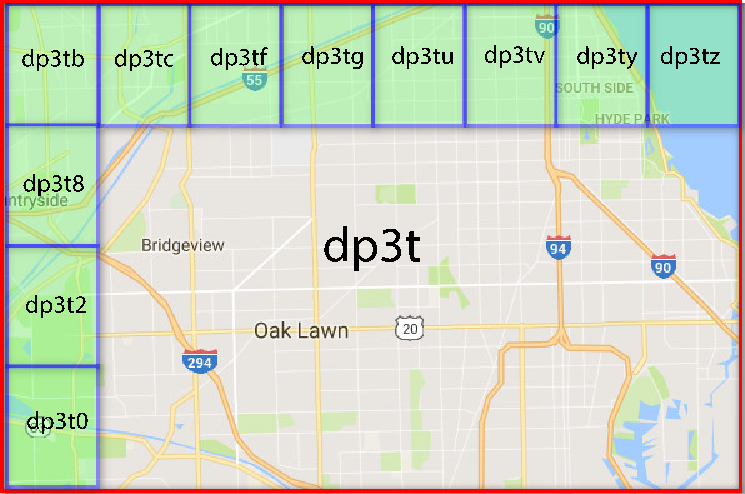
\includegraphics[width=0.35\textwidth]{./figures/geohash.pdf}
    \caption{Geohash method overview}\label{fig:geohash}\vspace{-0.1in}
\end{figure}

Our idea is that only the locations in a certain region represented by one Geohash can be inserted into an identical bloom filter labeled by this Geohash, i.e., any locations outside this region are never allowed to inserted into this bloom filter. Possible largest areas (the areas decrease from the equator to the poles) covered by different Geohash lengths are illustrated in Table \ref{tab:geohash_region_size}. Because the region size of the Geohash length of 4 is so large, the bloom filter size has to be very large to contain all possible locations in this region, and the region size of the Geohash length of 6 is so small that it is easy to guess users' locations once the Geohash becomes available. So, normally we take the Geohash length of 5 to identify a bloom filter, i.e., all the locations within a certain region of 4.89km x 4.89km are inserted into a bloom filter. Note that the optimal Geohash length might depends on the environment. For example, a shorter Geohash length probably works very well in the desert areas or at sea, but on Manhattan Island a longer length can be used safely.

\begin{table}[]
\centering
\footnotesize
\caption{Metric Dimensions of the Region Covered by Different Geohash Lengths}
\label{tab:geohash_region_size}
\begin{tabular}{|c|c|c|}
\hline
Geohash Length & Region Width & Region Height \\
\hline
1 & 5,000km & 5,000km \\
2 & 1,250km & 625km \\
3 & 156km & 156km \\
4 & 9.1km & 19.5km \\
5 & 4.89km & 4.89km \\
6 & 1.22km & 0.61km \\
7 & 153m & 153m \\
8 & 38.2m & 19.1m \\
9 & 4.77m & 4.77m \\
10 & 1.19m & 0.596m \\
11 & 149mm & 149mm \\
12 & 37.2mm & 18.6mm \\
\hline
\end{tabular}
\normalsize
\vspace{-0.1in}
\end{table}

Suppose Bob queries the location of Alice. With the Geohash-based homomorphic bloom filter, Alice sends all her encrypted Geohash $E(G_a)$ to the aggregation server. Bob also submits his encrypted Geohash $E(G_b)$ to the server. Then the server checks whether the $G_b$ is in $G_a$ or not, by subtracting $E(G_b)$ from each element in $E(G_a)$, and sends the ciphertext results to Alice for decryption. Once Alice finds out no plaintext result equals 0, we can conclude that there is no intersection between Alice and Bob. Otherwise, Alice can identify the bloom filter $BF$ where Bob's location may exist by:


\begin{equation}
BF = \frac{\sum_{i = 1}^{s}G_{ai} - \sum_{i = 1}^{s}D(E(G_{ai}) - E(G_b))}{s}
\label{math:hash_lable}
\end{equation}




where $s$ is the size of $G_a$. Then all the protocols we mentioned before can be used for a further query.





\section{Implementation}
\label{sec:implementation}

In this section, we describe the implementation details and tradeoffs. We first describe the working flows of FHE. Then we describe the parameter selections.

\subsection{Working flows of fully homomorphic encryption (FHE)}

We implement our solution based on the Simple Encrypted Arithmetic Library (SEAL), which uses Fan-Vercauteren (FV) fully homomorphic encryption scheme \cite{fan2012somewhat}. The typical working flows of the FV scheme consist of the following six steps.

\subsubsection{Operand Encoding}

The first step is on encoding operands. As plaintext elements in the FV scheme are represented by polynomials, before being encrypted, the plaintext operands must be encoded as polynomials. Because all plaintext operands used in our approaches are integers, we choose the BinaryEncoder in SEAL, which encodes plaintext integers into a polynomials with a base of 2 and the corresponding coefficients are either 1 or 0.  For example, $26 = 1*2^{4} + 1*2^{3} + 1*2^{1}$, where the coefficient of $2^2$ is 0. After this step, all encodings will be finished.

\subsubsection{Key Generation}
In this step, we generate a pair of public key and private key. The public key, used to encrypt the plaintext data, may be available to multiple parties, while the private key for decryption must be kept confidential to its respective owner. For example, when Bob queries Alice's locations, the trajectories of Alice will be encrypted by the public key, but the results of the query will be decrypted by Alice using the corresponding private key. Note that other parties are not permitted to obtain Alice's private key.

\subsubsection{Encryption}
In this step, we use the public key to encrypt the encoded plaintext integers in step 1. Because of the security feature of FV scheme, different encrypted data will be created even with the same plaintext data and the same public key, i.e., there exist many ciphertexts per plaintext.

\subsubsection{Evaluation}
In this step, we perform arithmetic operations on encrypted operands and get the encrypted results. The major arithmetic operation we use is addition. In our approach, this step is performed on the server. Because the calculation results are ciphertexts, they leak no information to the server.

\subsubsection{Decryption}
In this step, we convert the private key to decrypt the results in step 4 into polynomials. This step can only be executed by the private key owner. Note that the decrypted results are still not plaintext but encoded polynomials.

\subsubsection{Operand Decoding}
We use the encoder, which must match the type of the encoder used in step 1, to convert the result polynomials in step 5 into plaintext. Therefore, we still use the BinaryEncoder in this step.

\subsection{Parameter selection for FV scheme in SEAL}
\label{sec:para_sele}

The following three parameters should be initialized before using FV scheme in SEAL.

\subsubsection{Polynomial Modulus}
This parameter determines the number of coefficients in encrypted polynomials. It must be a power of 2 cyclotomic polynomial in the form of $``1x \,\hat{}\, 2^n + 1"$, where $n\in\mathbb{Z}$ and $n \geq 10$ is recommended. Because the data involved in our protocols are not large, we set the $n$ as $10$, i.e, the polynomial modulus $``1x \,\hat{}\, 1024 + 1"$.

\subsubsection{Coefficient Modulus}
The ratio of this integer parameter over the plaintext modulus approximately stands for the upper bound on the maximum ``inherent noise'' tolerated by a ciphertext. A large coefficient modulus will increase the tolerable ``inherent noise'', but the bit size of coefficient modulus should not exceed a certain boundary determined by polynomial modulus \cite{lepoint2014comparison}. Otherwise, the ciphertext become impossible to decrypt. Actually, each polynomial modulus has a default value of coefficient modulus in SEAL. In our case, the coefficient modulus is set as $FFFFFFF00001$.

\subsubsection{Plaintext Modulus}
As mentioned above, the larger this parameter is, the smaller amount of ``inherent noise'' ciphertexts can tolerate. Compared with the homomorphic multiplication, the homomorphic addition causes the noise to increase much more slowly. However, in our solution, homomorphic addition is more often used. Besides, a larger plaintext modulus will support a better homomorphic integer arithmetic, which is widely used in our solution. Therefore, we set the plaintext modulus a relative large value of $256$.








\section{Security Analysis}
\label{sec:analysis}

As the goals of our system is to provide a secure and private protocol for users to share location data without leaking data, we now analyze the security of this system in the perspectives of Alice, Bob, and the aggregation server.

\subsection{Alice's Actions}

Observe that in our protocol designs, as long as Alice correctly encrypts her data with the public key, her security and privacy is well protected. Neither the aggregation server nor Bob has access to the plain text of Alice's positions. Therefore, users will not be discouraged from adopting this service and publishing their trajectories due to privacy concerns. 

On the other hand, Alice is able to decrypt the results received from the aggregation server in case there are intersections, which, in our practical protocols 1 and 2, contains the encrypted bloom filter positions of Bob. Theoretically, Alice is able to use her private key to find the true positions in Bob's bloom filter that have been flipped to $1$s. However, this does not pose a significant security challenge due to that Bob is using cryptohashing functions, which are impossible to reversely compute the locations based only on the hashed values. Furthermore, even if Alice may choose to cache such data, Bob is usually mobile and will not stay in the proximity of Alice for a long time. As soon as Bob moves out of the range of Alice, Alice is no longer to infer Bob is nearby, hence providing assurances on the privacy of Bob. 

Alice may also choose to broadcast fake location trajectories through the aggregation server, leading to non-existent intersections with other users. In such scenarios, Alice may be able to further contact Bob after this protocol, claiming the two users have intersections on query trajectories. We consider such a problem to always exist as users can always fake their GPS positions through software. Our protocol only ensures that Bob will not reveal true location through this protocol, but considers such further interactions to be out of scope of this protocol.

\subsection{Bob's Actions}

Because all data received by Bob are encrypted using the public key of Alice, and Bob does not own the private key, Bob does not gain any information on Alice's trajectory. Even the results on whether there are intersections are invisible to Bob. Therefore, we conclude nothing valuable is leaked to Bob.

Another action Bob can perform is to fake his locations. However, this would not give Bob any advantage because it is up to Alice to decide whether to further contact after the protocol finishes. Furthermore, as Bob does not know the location of Alice, it is practically impossible to choose a location that happens to have intersections with Alice's in a short time. 

In the protocol based on the geohash system, it will inherit the security properties of protocols 1 to 3. As the number of possible geohash strings is limited, this protocol may leak the area of the queried location belonging to Bob. However, as long as the granularity of the geohash system is carefully chosen, such information leak will be limited and does not compromise the security of the whole system.

\subsection{The Aggregation Server}

We assume that the messages between Alice, Bob, and the server are encrypted, so the communication channel can be secure. On the other hand, even if the server is able to read and write all messages, information is not leaked to the server due to the very nature of the homomorphic encryption: all computations are based on encrypted data, not plain text. 

On the other hand, the server indeeds is able to log the IP addresses and user accounts of the users. But we consider this not a security problem as this is the standard operations of social networks and apps. Finally, the server may sabotage the system by refusing to act as the intermediate server. In practice, this does not happen often as servers lack the motivations to block users arbitrarily. 
 
%\section{Discussion}
\label{sec:discussion}
\section{Evaluation}
\label{sec:evaluation}

In this section, we report experimental results of our homomorphic bloom filter protocols based on a real-world mobile data access dataset. First, we briefly describe the dataset and the experimental setup. Next, the parameter settings of the protocols used in our experiments are presented. Then, we compare the computation and communication overhead of different protocols. Finally, we explore the impacts of Geohash length on the computing efficiency as well as the security.

\subsection{Datasets and Experimental Setup}
Our dataset consists of multiple mobile data access traces of smartphone users in a small city in China. More specifically, this dataset includes 7607 unique users, 121 cell towers, and is collected from 6:00 pm to 9:00 pm on a Sunday in 2014. Each mobile data access record contains the coordinate of the cell tower with which the user communicates. A sequence of records of a user can be viewed as her history trajectory. We randomly pick users and generate queries for evaluation. All experiments are performed on a PC with a 3.10GHz Xeon E3-1220 processor, and 32GB memory,
running Red Hat 4.8.5.

\begin{figure*}[t]
	\centering
	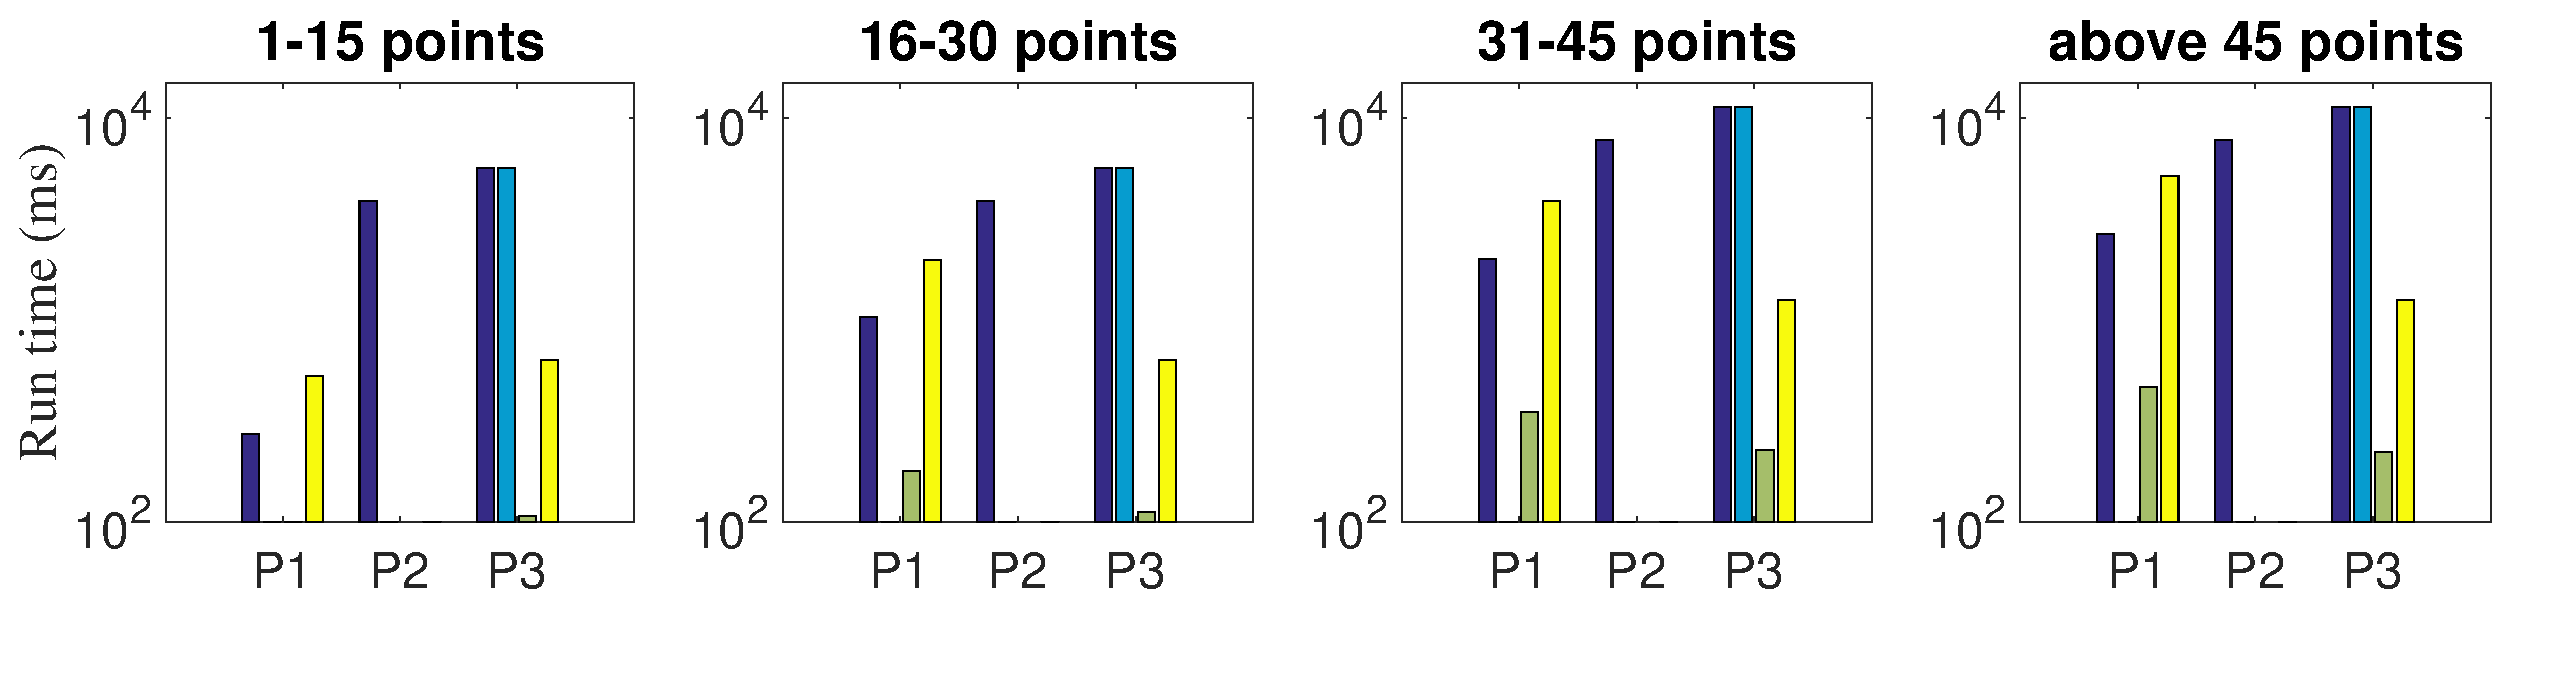
\includegraphics[width=\linewidth]{figures/computation_oh.pdf}
	\caption{Computation overhead.}
	\label{fig:computation_oh}
\end{figure*}

\subsection{parameter settings}
We group users in our dataset into 4 categories, by their number of unique visited location points: 1-15 points, 16-30 points, 31-45 points, above 45 points. According to number of unique location points of each group, we set the bloom filter parameters according to~\autoref{equ:k} and~autoref{equ:m}. The desired false positive probability is set as 0.1. We use 250 bit bloom filter with 4 hash function for group 1 \& 2, i.e., users with fewer visited location points than 30. We use 500 bit bloom filter with 4 hash function for group 3 \& 4, i.e., users with more visited location points than 30.

We implement our design both on an integer encryption system (SEAL) and a binary encryption system based on ~\cite{van2010fully}. More specifically, Protocol 1 and Protocol 2 are implemented on integer encryption system, while Protocol 3 is implemented on binary encryption system. As mentioned in \ref{sec:para_sele}, we set polynomial modulus as $``1x \,\hat{}\, 1024 + 1"$, coefficient modulus as $FFFFFFF00001$ and plaintext modulus as $256$. Under this setting, we calculate the size of a freshly encrypted integer in SEAL as $1025*48*2 = 98400$ bits, where $1025$ is the number of coefficients in one polynomial, $48$ is the number of bits per coefficient occupies, and $2$ is the size of the array of polynomials. To minimize difference of the size of cipertext, for binary encryption system, the security parameter $\lambda$ is set as 4, and each bit in the plaintext is encrypted into 1024-bit wide ciphertext.

\subsection{computation overhead}
The computation overhead can be decomposed to three part: the encryption time, the query computation time and decryption time, where encryption happens at both A and B. We randomly perform 20 queries for each group of users and compare the computation overhead of all three protocols in \autoref{fig:computation_oh}. 

As you can see that in protocol1 (P1) encryption overhead at A is much larger than encryption overhead at B as the number of integers to be encrypted relates to the number of elements inserted into the bloom filter. Such a relation is also the reason why the encryption overhead increase as the number of location points increase. Since protocol1 also incur large intermediate results to be transmit back to A, so the decryption overhead is also very high which can reach 5 seconds. In protocol2 (P2), the encryption overhead at A dominates the overall computation overhead which can reach 8 seconds. As the data at B and intermediate results are both very short. The computation overhead of protocol3 (P3) can reach 24 seconds in total (11 seconds for encryption) which is the highest among all three protocols, mainly because the encryption method is different (bitwise encryption). All three protocols show a same trend is that the computation overhead are mainly caused by encryption/decryption whereas the query computation has very limited contribution towards the overall computation overhead.

\subsection{communication overhead}
The communication overhead consist of three parts: send ciphertext from A and B to server, retrieve computation results from cloud to A, A send query result to B. Since the last part is transmitted in plaintext and the size is negligible, so we focus on the first two parts in our evaluation. 

We use the size of the ciphertext to be transmitted as the main measure for communication overhead. We compare the communication overhead of all three protocols in \autoref{fig:communication_oh}.

\begin{figure*}[h]
    \centering
    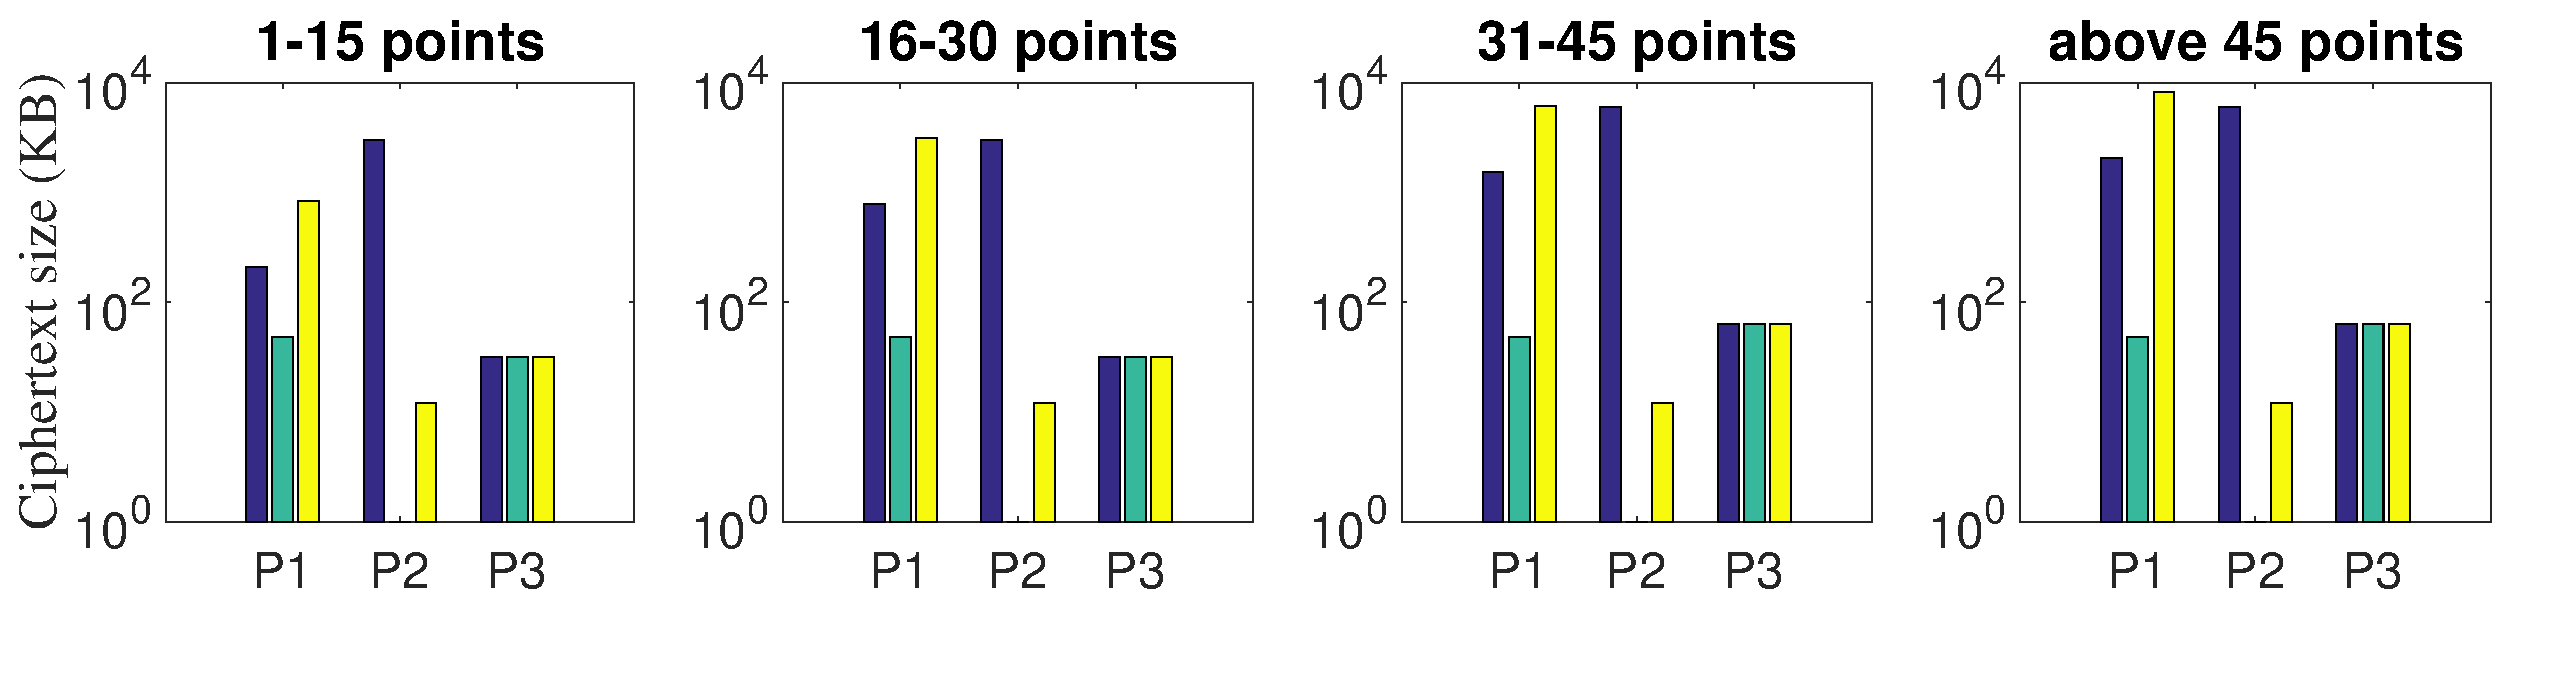
\includegraphics[width=\linewidth]{figures/communication_oh.pdf}
    \caption{Communication overhead.}
    \label{fig:communication_oh}
\end{figure*}

As you can see that in protocol1 (P1), beside large communication overhead at transmitting ciphertext form A to server, the communication overhead of transmit intermeidate results are also very high as large number of ciphertext is created by the query computation. The highest overhead reaches 2MB. For protocol2 (P2), most of the overhead happens at sending ciphertext from A to server, as each bit in the bloom filter is treated as an integer. The communication overhead of protocol2 is the highest among all three protocols which can reach 6MB. Protocol3 (P3) which adopts a bitwise encryption scheme, has the lowest communication overhead with only tens of KB in size. 

\subsection{the accuracy}
As the bloom filter has possible false positives. We evaluate here the with different required false positive possibility $p$, how are the overhead changes. We show the trend of the computation overhead in \autoref{fig:accuracy_comp} and the communication overhead in \autoref{fig:accuracy_comm}.

For protocol1 (P1), we can see that the both computation overhead and communication overhead mainly decreases as $p$ increases with the exception that the encryption overhead at B is stable as it require constant time. For protocol2 (P2), as the encryption at A and transmit data from A to server dominate the computation overhead and communication overhead respectively, they both decreases as $p$ increases, where as other overheads are quite stable. Similar to protocol1 and protocol2, protocol3 also shows a trend of decreasing overhead as $p$ increase.

\begin{figure*}[h]
    \centering
    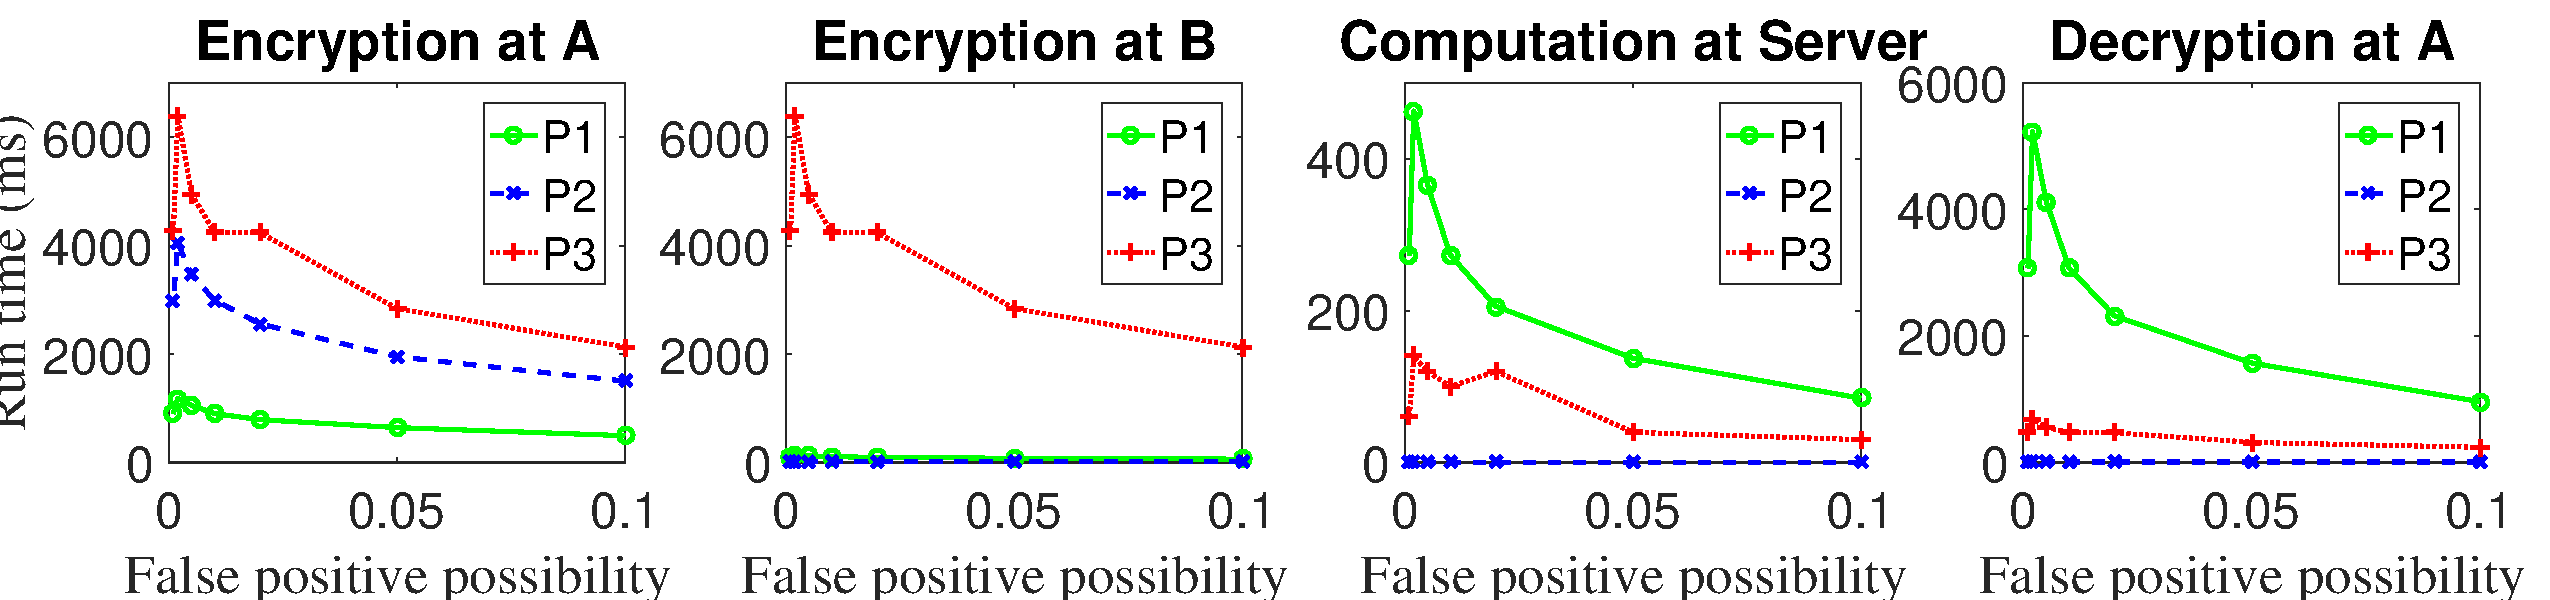
\includegraphics[width=\linewidth]{figures/accuracy_comp.pdf}
    \caption{Accuracy vs computation overhead.}
    \label{fig:accuracy_comp}
\end{figure*}


\begin{figure*}[h]
    \centering
    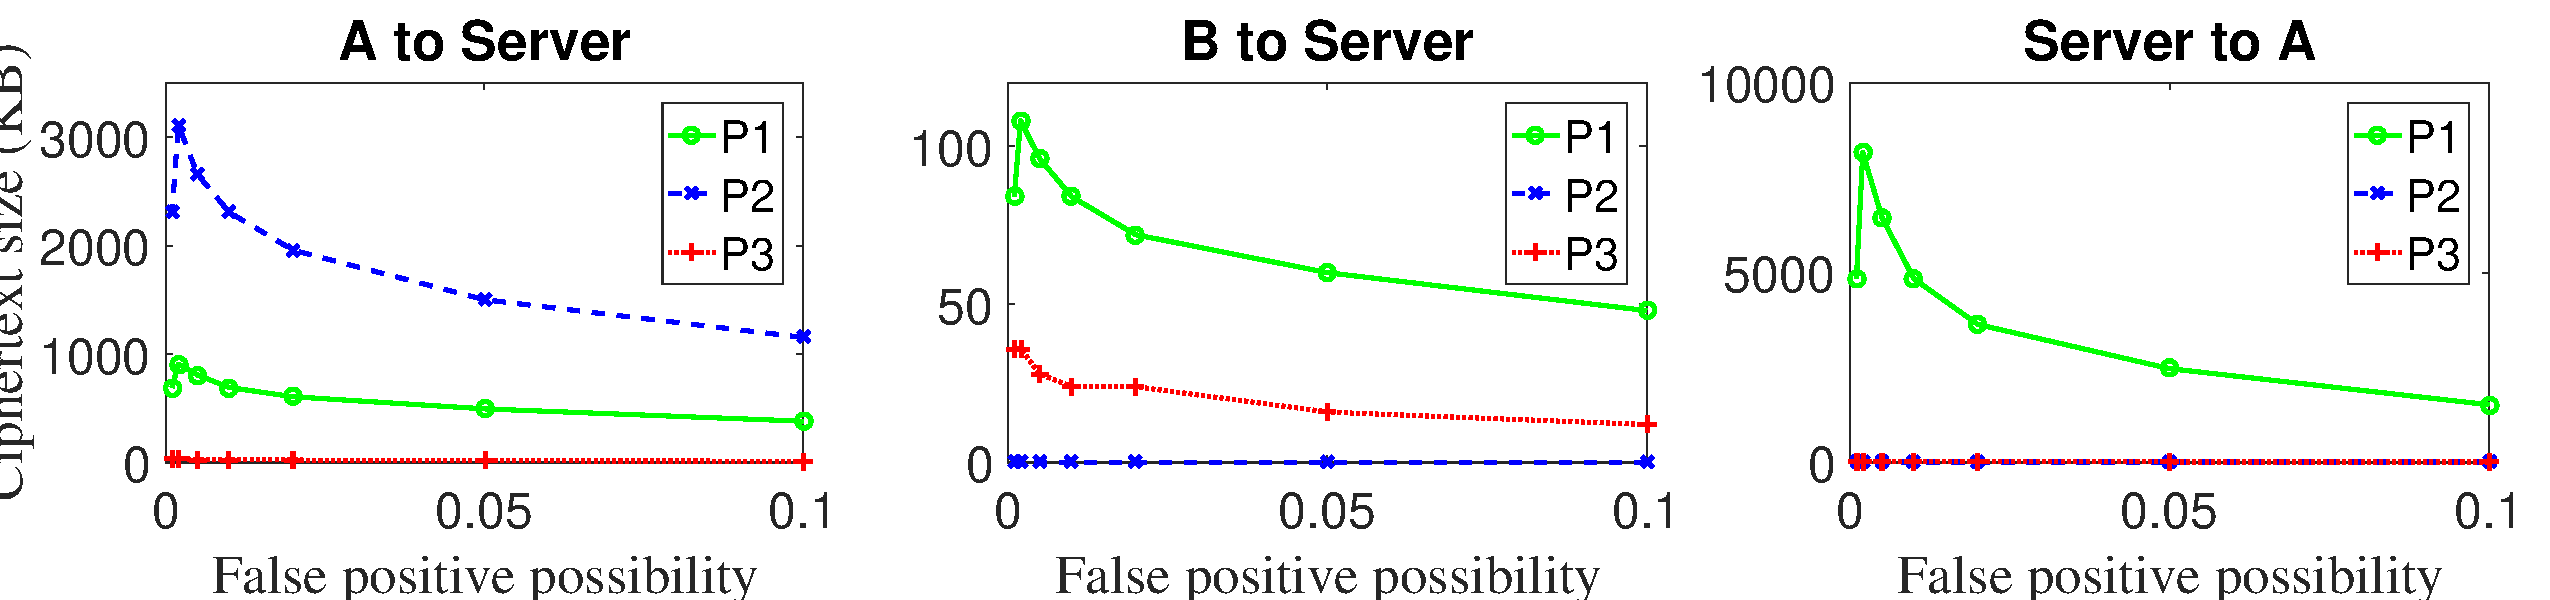
\includegraphics[width=\linewidth]{figures/accuracy_comm.pdf}
    \caption{Accuracy vs communication overhead.}
    \label{fig:accuracy_comm}
\end{figure*}

\subsection{geohash efficiency}
Geohash help to reduce both computation overhead and communication overhead compared to regular version. We evaluate the relation of the size of regions and reduction in overheads. Various region size are used and results are shown in \autoref{fig:geohash}.

By sending geohash values in plaintext, B also possibly reveal his location information to A. The possibility of reveal the exact location highly related to the number of location points in each region.

Figure \ref{fig:geohash_eval} illustrates the bloom filter size required to keep the false positive rate $p$ not larger than 0.01, and the probability of leaking private locations during the query with various Geohash lengths. We assume the locations are evenly distributed and there is exactly one location distributed in the area of 1m x 1m, 10m x 10m, 100m x 100m and 1km x 1km respectively. Take the 1m x 1m and the Geohash length of 6 as an example. Since exactly only one location in each 1m x 1m area, the Geohash with a length of 6 covers an area of 1.22km x 0.61km, which can be found in Table \ref{tab:geohash_region_size}, containing $n$= 1220x610 locations, i.e., elements. Therefore, the size of bloom filter can be calculated by Equation \ref{equ:m}, and the probability of leaking the location can be expressed by $1/n$;

\begin{figure}[h]
    \centering
    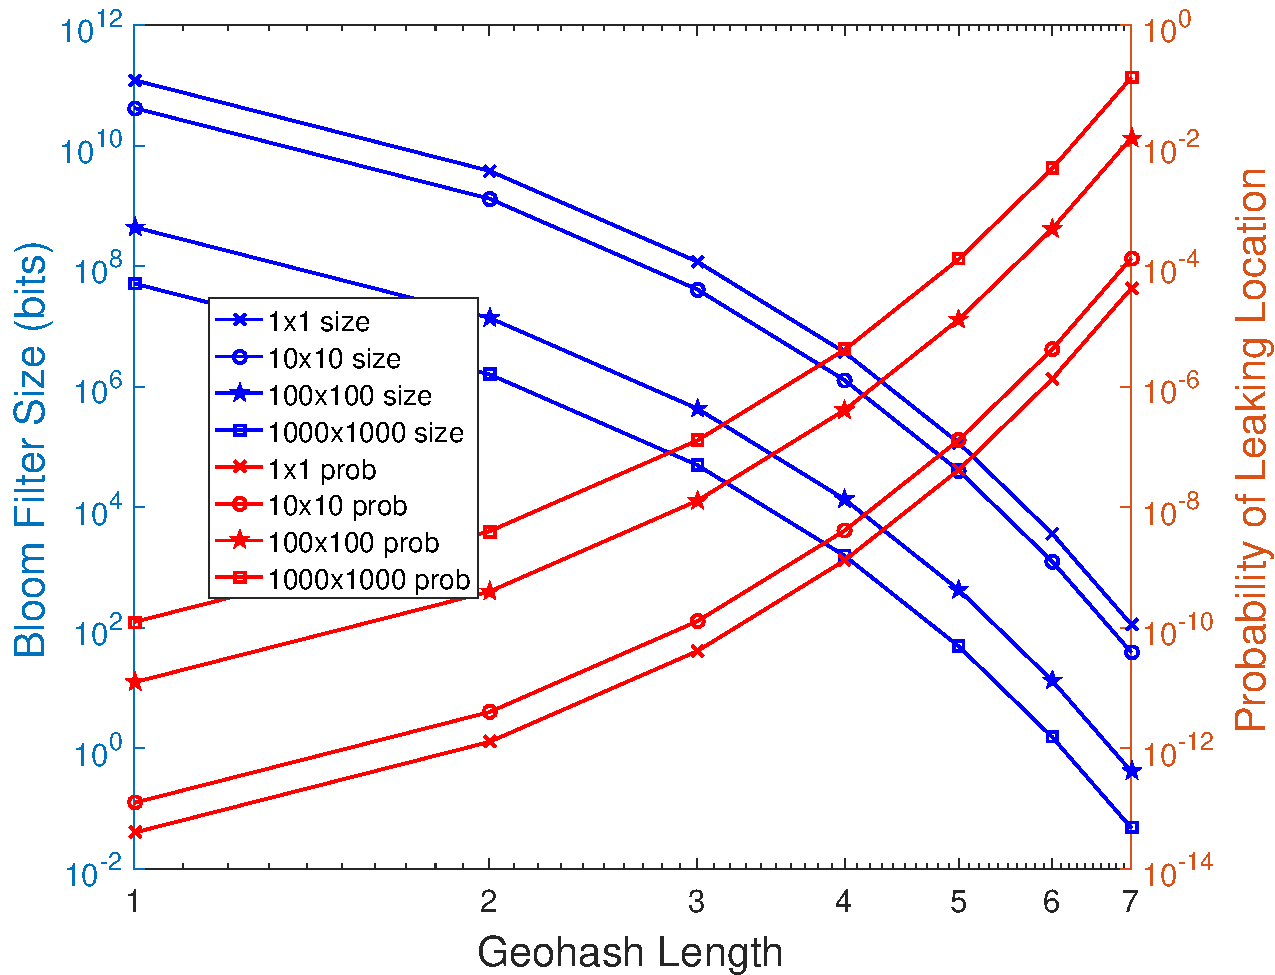
\includegraphics[width=0.7\linewidth]{figures/geohash_eval.pdf}
    \caption{Geohash.}
    \label{fig:geohash_eval}
\end{figure}


\section{Conclusion}
\label{sec:conclusion}

In this paper, we investigate the problem on how to keep users' location data secure, while at the same time allowing servers to perform basic operations on the data. We demonstrated secure computation primitives on location data where the servers should have no knowledge on the plaintext, i.e., the servers should not even keep the private keys to decrypt data. In this way, compromised servers will not cause leaked user data. Our work is built on the recently developed homomorphic computing principles, and developed a generalized secure set membership check framework based on an advanced data structure called the bloom filter. Our work, to our knowledge, is the first to propose a homomorphic version of this data structure. Finally, we also evaluated a working prototype, which is implemented on the open-source homomorphic libraries. Our preliminary results demonstrate the feasibility of the proposed approach as well as the security of the protocol designs. 

{
\bibliographystyle{IEEEtran}
%\bibliography{./biblio.bib}
\bibliography{biblio}
}

% that's all folks
\end{document}
